\documentclass{vldb}

\usepackage{graphicx}

\usepackage{times}

\usepackage{amsmath}

\usepackage{verbatim}
\usepackage{epsfig}
\usepackage[iso]{umlaute}
\usepackage{amssymb}
\usepackage{graphicx}
\usepackage{bbm}
\usepackage{subfigure}
\usepackage{ifthen}
\usepackage{url}
\usepackage{algorithm}
\usepackage{color}
\usepackage{marginnote}

\usepackage{algorithm}
\usepackage{algorithmic}
\usepackage{paralist}
\usepackage{tabularx}
\usepackage{ifthen}
\newcommand{\DB}{\ensuremath{\mathcal{D}}}
\newcommand{\db}{\ensuremath{\mathcal{D}}} %the database
\newcommand{\NN}{\ensuremath{\mathbb{N}}}
\newcommand{\RR}{\ensuremath{\mathbb{R}}}
\newcommand{\statevec}{\ensuremath{\vec{s}} }
\newcommand{\query}{\ensuremath{q} } %the query object
\newcommand{\loc}{\ensuremath{x} } %a single location
\newcommand{\sd}{\ensuremath{\mathcal{S}}} %spatial domain
\newcommand{\td}{\ensuremath{\mathcal{T}}} %time domain
\newcommand{\tint}{\ensuremath{t} }
\newcommand{\dbobj}{\ensuremath{o} }
\newcommand{\vardbobj}{\ensuremath{g}}
\newcommand{\vart}{\ensuremath{h}}
\newcommand{\tm}{\ensuremath{M}} %transitionmatrix
\newcommand{\probm}{\ensuremath{J}}
\newcommand{\pw}{\ensuremath{\bullet}} %piecewise multiplication
\newcommand{\mm}{\ensuremath{\cdot}} %matrix multiplication
\newcommand{\tpoint}[1]{\ensuremath{\mathbb{#1}} }
\newcommand{\plusequal}{\ensuremath{{ + \atop =}}}
\newcommand{\obs}{\ensuremath{ob}}
\newcommand{\CP}[1]{{\color{red}#1}}
\newcommand{\TODO}[1]{{\bfseries\color{red}TODO: #1}}

\newtheorem{theorem}{Theorem}[section]
\newtheorem{definition}{Definition}
\newtheorem{lemma}{Lemma}
\newtheorem{corollary}{Corollary}
\newtheorem{example}{Example}

\graphicspath{.}
\newboolean{TR}
\setboolean{TR}{false}
\renewcommand{\textfraction}{0.00}
\renewcommand{\topfraction}{1.0}
\renewcommand{\bottomfraction}{1.0}
\setcounter{totalnumber}{100}
\setcounter{bottomnumber}{100}
\setcounter{topnumber}{100}


\title{On Task Assignment in Spatial Crowdsourcing}
\begin{document}
\numberofauthors{1}
\author{{}\\
\\
\fontsize{10}{10}\selectfont\rmfamily\itshape
$~^{*}$Integrated Media Systems Center, University of Southern California\\
\fontsize{9}{9}\selectfont\ttfamily\upshape
\{\}@usc.edu\\
}
\maketitle
\begin{abstract}
\cite{kazemi12}
\end{abstract}

\vspace{-0.2in}
\section{Introduction}
\vspace{-0.1in}

Smartphones are ubiquitous: we are witnessing an astonishing growth in mobile phone subscriptions. The International Telecommunication Union estimates there are nearly 7 billion mobile subscriptions worldwide. Meanwhile, the mobile phones' sensors (e.g., cameras) are advancing and the network bandwidth is constantly increasing. Consequently, every person with a mobile phone can now act as a multi-modal sensor, collecting and sharing various types of high-fidelity spatiotemporal data instantaneously (e.g., picture, video, audio, location, time, speed, direction, and acceleration).

Exploiting this large crowd of potential workers and their mobility, a new mechanism for efficient and scalable data collection has emerged: Spatial Crowdsourcing (SC) \cite{Kazemi12}. Spatial crowdsourcing requires workers (e.g., willing individuals) to perform a set of tasks by physically traveling to certain locations at particular times. Spatial crowdsourcing is exploited in numerous industries, e.g., Uber, TaskRabbit, Waze, Gigwalk, etc., and has applications in numerous domains such as citizen-journalism, tourism, intelligence, disaster response and urban planning. With spatial crowdsourcing, a requester submits a set of spatiotemporal tasks to a spatial crowdsourcing server (SC-Server). Subsequently, the SC-Server has to select a worker to perform each task.

Different studies on spatial crowdsourcing \cite{Kazemi12,Li15,Deng15,Chen15,Cheng16,Fonteles15,Guo16} can be classified based on two basic characteristics of the problem; (1) whether the problem \textit{matches} a task with a worker and (2) whether the problem \textit{schedules} matched tasks for the workers. Early studies in SC \cite{Kazemi12,Fonteles15,Cheng16} used a \textit{scheduling-oblivious-matching (SOM)} approach where tasks are matched with workers without considering the workers' schedule. Assuming the tasks have already been matched with workers, other studies. \cite{Deng13,Li15} study the problem of  scheduling the tasks that have been assigned to a worker. They show that there is no guarantee that the worker could schedule all of its matched tasks. We argue that with Spatial Crowdsourcing, it is not enough to only \textit{match} a task with a worker. An SC-Server must consider the \textit{schedule} of every worker when matching a task to workers and only consider those workers who are able to fit the task in their schedule. In this paper, we define the task assignment problem in SC consisting of two phases, a matching phase and a scheduling phase, which need to happen in tandem. Neither of these phases should be ignored, otherwise, the resulting solution is rendered infeasible for real-world applications.

More recent studies consider both matching and scheduling in spatial crowdsourcing \cite{Deng15,Chen15,Guo16}. These studies utilize a \textit{batched assignment} scheme, where the assignment is delayed for a period of time (i.e., batching time interval) during which all the arrived tasks are batched to be matched and scheduled during the next time interval. Once the tasks are batched and processed together, suddenly the matching phase becomes complex because many tasks need to be matched to many workers. This in turn adds to the running time and increases the batching time interval. 
%Consequently, neither studies can support real-time assignments.

%(3) whether the problem requires \textit{real-time} results where the task requester is notified within a few seconds whether his task will be executed or not. For example, an Uber user requesting a ride, does not want to wait for 10 minutes to find out if a driver is available or not.

A long batching time interval (e.g., 10 minutes) has two main disadvantages.  First, the duration of the batching time interval should be subtracted from the tasks' deadline, leaving each task with less available time to be scheduled. Second, batch scheme can no longer generate real-time assignments. While there might be cases where a real-time assignment is not required, there are many other real-world applications where real-time assignments are a necessity; For example, an Uber user requesting a ride, does not want to wait for 10 minutes to find out if a driver is available or not. Contrary to batched assignment, in \textit{online assignment}, a task is assigned to a worker as soon as it arrives at the SC-Server. This requires the server to perform matching and scheduling in real-time. With online assignment, at each point of time the SC-Server is processing only one task and hence, the matching phase becomes a one-to-many matching where there are multiple workers and only one task. Consequently, the complex many-to-many matching phase of batched assignment is reduced to only selecting the best worker that can fit the task in its schedule. Even though matching is fast with online assignment, the server must still perform scheduling for multiple workers. Therefore, the scheduling phase becomes the bottleneck in online assignment. As shown in \cite{Li15}, scheduling for a single worker can be performed fast. However, an online monolithic\cite{Stephens15} SC-Server (monolithic-SC), where the server has to schedule only a single task for \emph{all} workers, is not capable of processing tasks in real-time. For example, in New York City, during rush hours, there are as many as 10+ ride requests per second \cite{NYCTaxi}. Through experiments, we show that monolithic-SC is not able to support such throughput in real-time. Towards this end, we propose Auction-SC: an auction-based framework for real-time task matching and scheduling. Similar to monolithic-SC, Auction-SC is an online framework where tasks get matched with workers as soon as they become available and hence, the matching phase is fast. Moreover, we overcome the scheduling bottleneck by distributing it among the workers.

With Auction-SC, the server broadcasts a task to the workers upon the task's arrival. Each worker\footnote{Hereafter, we use the term "worker" interchangeably to refer to both the human worker and the software running on her mobile device unless clear distinction is needed.} submits a bid for that task based on its current schedule and location. To compute its bid, each worker has to consider only its own schedule so the bid computation phase can be done in real-time. Once every worker submits its bid to the SC-Server, matching the task to a worker reduces to selecting the highest bid.

We introduce a branch-and-bound scheduling algorithm where for each new task, the worker performs an exhaustive search to find out whether it can fit the incoming task into its schedule. We show that at each point of time the number of remaining tasks for each worker (the number of tasks that the worker has scheduled and not completed yet) is in a range that even the branch-and-bound algorithm can be completed in real-time. However, in our experiments, we show that even replacing the branch-and-bound algorithm with a polynomial time approximate algorithm, will not affect the quality of the assignment significantly.

%In addition to the branch-and-bound algorithm, we propose a more complex bidding technique that considers the probability of a task appearing in a spatial region in the future. The key idea is that having more workers in areas where there is a higher chance of having tasks in the future, can increase the quality of the assignment. This consideration increases the complexity of the bid computation phase such that it may impact the scalability of the framework. However, we show that the SC-Server can still manage a throughput of \textasciitilde 50 tasks per second with this complex bidding technique.

We conduct many experiments on both real-world and synthetically generated workloads to evaluate different aspects of Auction-SC. For our real world data we use two geo-social datasets (Gowalla \& Foursquare). First, we show that compared to Auction-SC, both the SOM and batched approach result in a much lower assignment rate as a result of ignoring scheduling while matching and long batching intervals, respectively. Subsequently, we show that when matching and scheduling are performed in tandem, neither the batched scheme nor the online monolithic SC-Server can process more than 5 tasks per second. However, with the auction based framework, the throughput of the system increases by orders of magnitude.

In sum, the contributions of this paper are as follows:

\begin{itemize}
\item We formally define the \textit{online} task assignment problem in SC and analyze its complexity.
\item We introduce the Auction-SC framework as a scalable solution for the online task assignment problem in SC. 
\item We propose a novel algorithm for computing bids in Auctions-SC where both the spatial and temporal dynamism of SC are considered.
\item Through experiments on real-world and synthetic data, we show Auction-SC outperforms alternative approaches in the number of completed tasks and scalability.
\end{itemize}
%\item Through various experiments on real-world and synthetic data, we show (1) a larger number of tasks are completed with Auction-SC as compared to both the batched and SOM approaches and (2) unlike Auction-SC, neither the batched nor the online Monolithic-SC approaches can scale to real-world requirements.

The remainder of this paper is organized as follows. In \cref{sec:prelim} we formally define the online task assignment problem in SC and discuss its complexity. We review the related work in \cref{sec:related}. We introduce Auction-SC in \cref{sec:onlinealgo} and propose a novel bidding rule within the auction-based framework. We show the results of our experiments on both real-world and synthetic data in \cref{sec:experiments} and conclude the paper with guidelines for future work (\cref{sec:future}).

\vspace{-0.15in}
\section{Preliminaries}
\label{sec:prelim}
\vspace{-0.05in}
In this section, we define the terminologies used in the paper and provide a formal definition of the problem under consideration. In addition, we analyze the complexity of the problem and its hardness.
\vspace{-0.1in}
\subsection{Problem Definition}
\label{subsec:problemdef}
\vspace{-0.05in}
We start by defining some terminologies in order to formally define the task assignment problem in spatial crowdsourcing.
\vspace{-0.05in}
\begin{definition} [Spatial Task]
A spatial task t shown as $\left\langle l, [r, d] \right\rangle$ is a task to be performed at location l with geographical coordinates, i.e., latitude and longitude. The task becomes available at r (release time) and expires at d (deadline).
\end{definition}
\vspace{-0.05in}
It should be pointed out that in a spatial crowdsourcing environment, a spatial task \emph{t} can be executed only if a worker is at location \emph{t.l}. For example, if the query is to report the traffic situation at a specific location, someone has to actually be present at the location to be able to report the traffic. Hereafter, whenever we use \emph{task} we are referring to a spatial task. Now, we formally define a worker.
\vspace{-0.05in}
\begin{definition} [Worker]
A worker w shown as $\left\langle l, T, max, [s, e] \right\rangle$ is any entity, e.g., a person, willing to perform spatial tasks. We show the current location of the worker by w.l. Each worker has a list of tasks assigned to it, w.T, and a maximum number of tasks it is willing to perform, w.max. Also w.s and w.e show the availability of the worker such that the worker is available during the time interval $\left( w.s, w.e \right]$.
\end{definition}
\vspace{-0.05in}
Throughout the paper, we assume every worker moves one unit of length per unit of time. Therefore, we can assume that $distance \left( a,b \right)$ is also the \emph{time} required to move from point $a$ to point $b$.
\vspace{-0.05in}
\begin{definition} [Schedule]
We call an ordered list of tasks a schedule. We show s as $\left\langle t_1, ..., t_n \right\rangle$ where n is the number of tasks in s. If we show the $i^{th}$ task in s with $s^i$, we say worker w is able to perform schedule s if and only if:
\vspace{-0.05in}
\begin{equation*}
\forall i, 1\leq i \leq n \ \ \ \ \sum_{j=1}^i distance(s^{j-1}, s^j) \leq s^i.d - t_0
\vspace{-0.1in}
\end{equation*}
where $s^0$ and $t_0$ represent the current location of $w$ and current time respectively.
\end{definition}
\vspace{-0.05in}
At each point in time, a worker $w$ is associated with a schedule ($s_w$) and completes the tasks based on their order in its schedule.
\vspace{-0.05in}
\begin{definition} [Matching]
Assuming we have a set of workers W and a set of tasks T, we call $M \subset W \times T$ a matching if for each $t \in T$ there is at most one $w \in W$ such that $\left( w, t \right) \in M$. We call $\left( w, t \right) \in M$ a \emph{match} and say t has been matched to w. For each matching M, we define the value (benefit) of M as:
\vspace{-0.05in}
\begin{equation*}
Value(M) = \vert M \vert
\vspace{-0.1in}
\end{equation*}
\end{definition}
\vspace{-0.05in}
\begin{definition} [Valid Matching]
A matching $M$ is valid if and only if, for every worker $w$, there exists a schedule $s_w$, such that $(w, t_i) \in M \implies t_i \in s_w$. 
\end{definition}
\vspace{-0.05in}
Now we can formally define the Task Assignment in Spatial Crowdsourcing (TASC) as follows:
\vspace{-0.05in}
\begin{definition} [Task Assignment in SC]
Given a set of workers $W$, a set of spatial tasks $T$ and a cost function $d: \left( W \cup T \right) \times T \rightarrow \mathbb{R}$ where $d \left( a,b \right)$ is the distance between $a$ and $b$, the goal of the TASC$\left\langle W, T, d \right\rangle$ problem is to find a valid matching $M$ with maximum value.
\end{definition}
\vspace{-0.05in}
It is important to note that with task assignment in SC, the goal is to find a \textit{valid matching}. This means that in addition to finding a \textit{matching} between tasks and workers, the SC-Server has to also find a \textit{schedule} for each worker to perform the tasks. Throughout this paper we use the terms \textit{matching phase} and \textit{scheduling phase} to refer to the two different aspects of task assignment in SC.

In a real life scenario, the SC-Server only finds out about the exact properties of tasks once they are submitted. Similarly, the server does not know when future workers will become available. Consequently, a real-world SC-Server can either process every single task as soon as it becomes available (Online) or periodically wait for a specific duration and process all the tasks that have been submitted during that time (Batched). In this paper, we study the \textit{OnlineTASC} problem, where the server processes an incoming task as soon as it is submitted by the requester.
\vspace{-0.1in}
\subsection{Complexity Analysis}
\vspace{-0.05in}
Previous studies have shown the TASC problem is NP-Hard \cite{Deng15}. However, the focus of this study is the OnlineTASC problem and thus, in this section we briefly discuss the complexity of OnlineTASC.

In order to analyze online algorithms, where each request is processed without knowing the future, we use a method named \textit{competitive analysis}\cite{Sleator85}. With this method, the performance of an online algorithm is compared to the performance of an optimal offline algorithm that has knowledge of future events (clairvoyant). For the TASC problem, we measure the performance of each algorithm based on the number of assigned task. Assuming we show the performance of algorithm $\mathcal{A}$ on input $\mathcal{I}$ as $\vert \mathcal{A}\left( \mathcal{I} \right) \vert$ we can define \textit{competitive ratio} of an algorithm as:
\vspace{-0.05in}
\begin{definition} [Competitive Ratio]
For an online algorithm $\mathcal{A}$, we say $\mathcal{A}$ is c-competitive for some $c > 0$, if and only if:
\vspace{-0.1in}
\begin{equation*}
c = \min\limits_{\mathcal{I} \in \mathbb{I}} \left\lbrace \frac{\vert \mathcal{A}\left( \mathcal{I} \right) \vert}{\vert \mathcal{A}^{*} \left( \mathcal{I} \right) \vert} \right\rbrace
\vspace{-0.1in}
\end{equation*}
where $\mathcal{A}^{*}$ is the optimal offline algorithm and $\mathbb{I}$ is the set of all possible inputs.
\end{definition}
\vspace{-0.05in}
Now we can prove the following theorem regarding the complexity of OnlineTASC.
\vspace{-0.05in}
\begin{theorem}
\label{th:comp_ratio}
There does not exist a deterministic online algorithm for the OnlineTASC problem that is \textit{c-competitive} ($c > 0$). 
\end{theorem}
\vspace{-0.2in}
\begin{proof}
Suppose there exists an algorithm $\mathcal{A}$ that is \textit{c-competitive} for some $c \geq 0$. To prove no such algorithm exists, all we need to do is to prove there is at least one possible input ($\mathcal{I}$), for which $\frac{\vert \mathcal{A}(\mathcal{I}) \vert}{\vert \mathcal{A}^{*}(\mathcal{I}) \vert}$ is unboundedly small. For analyzing the \textit{competitive ratio} of a deterministic online algorithm $\mathcal{A}$, it is assumed that there exist an adversary which knows every decision $\mathcal{A}$ makes and creates an input knowing what decisions $\mathcal{A}$ is going to make. Here we show, how an adversary can generate an input for which the competitive ratio of any algorithm is unboundadly small. For simplicity, we only consider points on the x-axis and assume there is only one worker at point $x=0$ in the beginning.

The input starts with $t_1$ such that $t_1 = \left\langle 5, \left[0, 5 \right] \right\rangle$ (\cref{fig:prooft0}; a task at point $5$ with release time $0$ and deadline $5$). The algorithm can make two choices for the worker: (1) move towards $t_1$ or (2) stay still (in theory it can also make the worker  to move away from $t_1$ which in the context of this proof would be similar to case (2)). If choice 1 is selected, the adversary can generate the input such that at time $t = 2$, tasks $t_2, ... t_n$ are all submitted with the exact same properties as $\left\langle -4, \left[2, 7 \right] \right\rangle$ (\cref{fig:prooft21}). Considering that at the release time of $t2, ..., t_n$ the worker is at point $x=2$, it does not have enough time to get to $t_2, ..., t_n$ before their deadline. However, an optimal offline algorithm would have known about $t_2, ..., t_n$ in advance and would have ignored $t_1$ in order to be able to complete $n-1$ tasks instead. In other words, $\vert \mathcal{A} \vert = 1$ where $\vert \mathcal{A}^{*} \vert = n - 1$ and the ratio could be unboundedly small by increasing $n$. Therefore, we contradicted the assumption that $\mathcal{A}$ is \textit{c-competitive}. A similar argument can be made if choice 2 was selected by the algorithm by releasing tasks $t_2, ...,t_n$ with properties as $\left\langle 7, \left[2, 7 \right] \right\rangle$ (\cref{fig:prooft22}).
\end{proof}

\begin{figure}[h]
    \centering
    \subfigure[$t = 0$]{
        \label{fig:prooft0}
        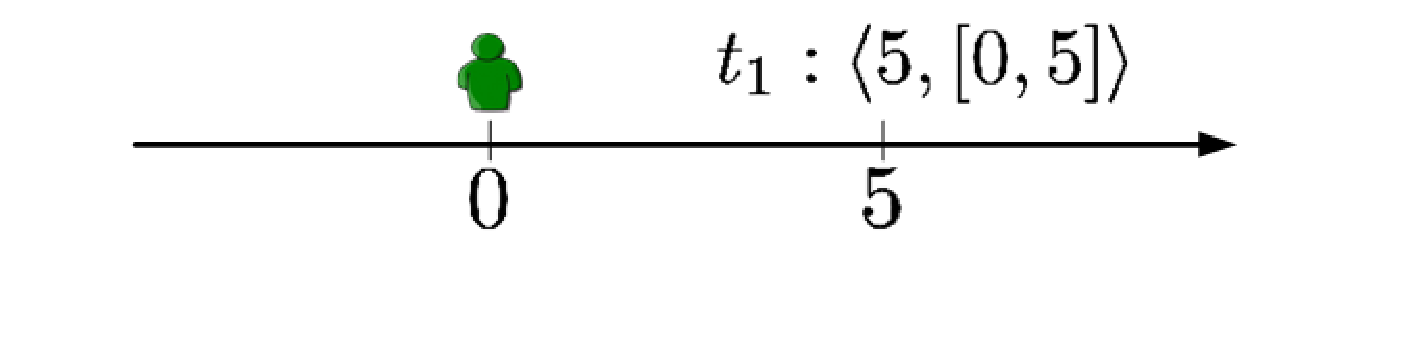
\includegraphics[width = 0.30\columnwidth]{figures/proof0}
    }
    \subfigure[$t = 2$, case $1$]{
        \label{fig:prooft21}
        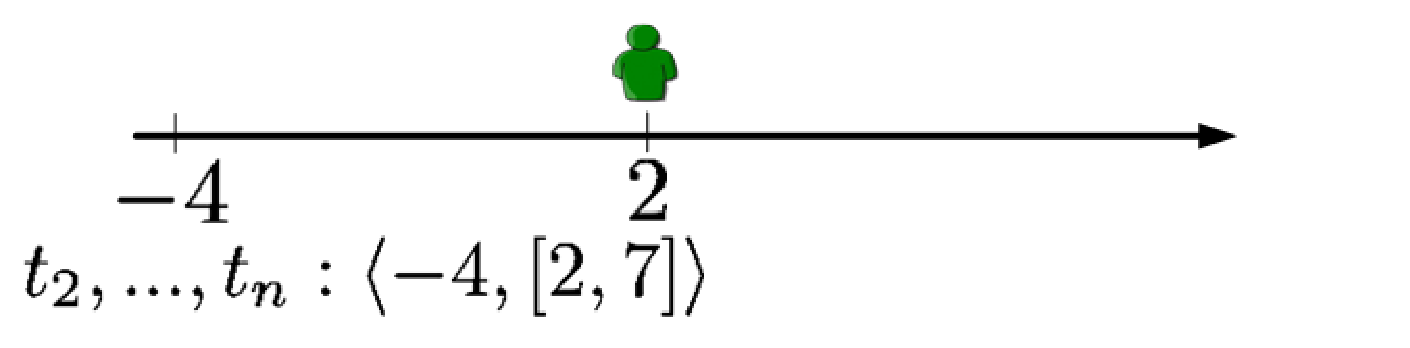
\includegraphics[width = 0.30\columnwidth]{figures/proof21}
    }
    \subfigure[$t = 2$, case $2$]{
        \label{fig:prooft22}
        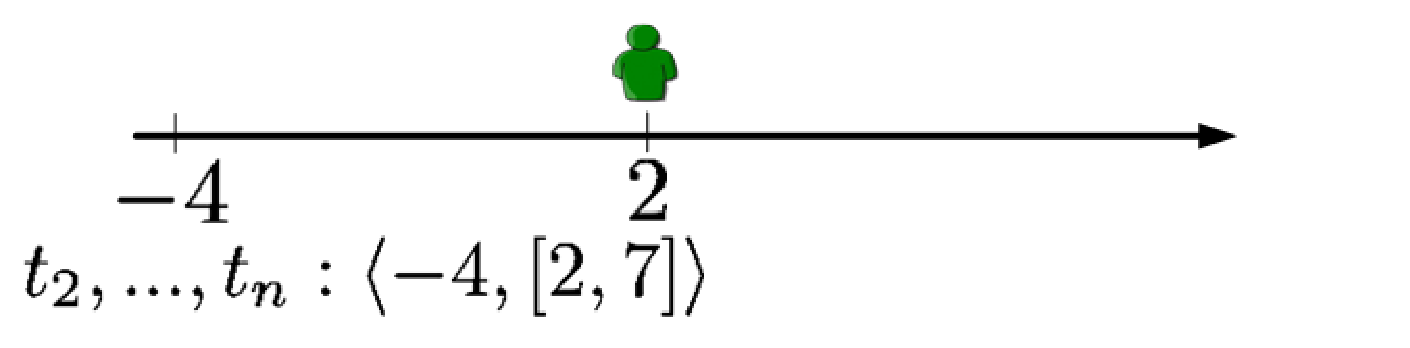
\includegraphics[width = 0.30\columnwidth]{figures/proof22}
    }
    \vspace{-0.15in}
    \caption{Adversary Generated Input}
    \label{fig:quality}
\end{figure}

\cref{th:comp_ratio} shows that for any deterministic online algorithm for OnlineTASC there exists a worst case scenario where the competitive ratio is very small and hence, there is no theoretical bound for the OnlineTASC problem. However, in the following sections we propose algorithms for OnlineTASC that generate close to optimal results when applied to both real-world and synthetic data.

%The equivalent decision problem for TASC is to decide if there exists a matching $M$ with value $K$ and is denoted as TASC$\left\langle W, T, d, K \right\rangle$. In this section we use a slightly modified version of the well known Hamiltonian Path Problem. We call it the Minimum Length Hamiltonian Path Problem (Min-Ham-Path) and define it as follows:

%\begin{definition}[Min-Ham-Path]
%Given a directed graph $G(V,E)$ where each edge $e \in E$ is assigned a length $l: E \rightarrow \mathbb{R}$, a source node $s$ and a length $L \in \mathbb{R}$, the Min-Ham-Path problem $\left\langle G, l, s, L \right\rangle$ is to decide whether there exists a path in $G$ that starts from $s$, visits every other node exactly once and has a length of at most $L$.
%\end{definition}

%\begin{theorem}
%\label{th:MinHam}
%The Min-Ham-Path problem is NP-Hard.
%\end{theorem}

%\begin{proof}
%Proof is shown in \cref{app:MinHamProof}.
%In order to prove the NP-Hardness of Min-Ham-Path we show Ham-Path $\leq_p$ Min-Ham-Path. The Hamiltonian Path problem asks the following question: Given a directed graph $G(V,E)$ does there exist a path that goes through every node exactly once?

%Given an instance of the Ham-Path problem $\left\langle G \right\rangle$ we modify graph $G(V,E)$ and generate a new graph $G'(V', E')$ where $V' = V \cup \left\{ o \right\}$ and $E' = E \cup \left\{ \left\langle o, v \right\rangle : v \in V \right\}$. Also, for every $e \in E'$ we Assume $l(e) = 1$.

%Now we show that Ham-Path$\left\langle G \right\rangle$ is true if and only if Min-Ham-Path$\left\langle G', l, o, n \right\rangle$ is true where $n$ is the number of vertices in $G$. If Min-Ham-Path returns a path of length $n$, we can remove the first edge from the path which results in a Hamiltonian Path for the Ham-Path$\left\langle G \right\rangle$ problem. On the other hand every Hamiltonian Path on graph $G$ has length $n-1$. By adding vertex $o$ and connecting it to the starting vertex, we end up with a Hamiltonian Path of length $n$ on $G'$.
%\end{proof}

%\begin{theorem}
%\label{th:TASC}
%The TASC problem is NP-Complete.
%\end{theorem}

%\begin{proof}
%Proof is shown in \cref{app:TASCProof}
%We start the proof by showing that the decision problem of TASC is \textit{verifiable} in polynomial time. Given a matching $M$, we can check that no task is assigned to more than one worker in polynomial time. Furthermore, based on the definition of a valid match, checking the validity of a matching $M$ can be done in polynomial time as well. Finally, we can find the value of $M$ by adding the value of every task in $M$.

%We show TASC is NP-Hard by proving the reduction Min-Ham-Path $\leq_p$ TASC. Given an instance of the Min-Ham-Path problem $\left\langle G(V,E), l, o, K \right\rangle$ we reduce it to an instance of the TASC$\left\langle W, T, l', n-1 \right\rangle$ problem such that $W = \left\{ o \right\}$, $T = V \setminus \left\{ o \right\}$. For every task $t$ we set $t.v = 1$, $t.r = 0$ and $t.d = K$. Also for every $e \in E, l'(e) = l(e)$. In addition for every $e' \in \left( W \times T \right) \cup \left( T \times T \right) $ where $e' \not\in E$ we set $l'(e') = \infty$.

%Finally we show the result of Min-Ham-Path$\left\langle G, l, o, K \right\rangle$ is true if TASC$\left\langle W, T, l', n-1 \right\rangle$ is true where $n$ is the number of vertices in $G$. Considering that $\left\vert T \right\vert = n - 1$ and $t.v = 1$ for every $t \in T$, if there exists a matching with size $n - 1$ it means every task has been assigned to the single worker. Also, since the deadline of every task is $K$ the worker visits every task no later than $K$. Therefore, the path that the worker traverses starts at $o$ and goes through every other vertex $v \in V \setminus \left\{ o \right\}$, where the length of the path is no more than $K$.
%\end{proof}

\section{Related Work}

Related Work

\section{Exact Clairvoyant Algorithm}
\label{sec:exactalgo}

% In a real world crowdsourcing environment, the server has no information with regard to tasks (workers) becoming available in the future. The server becomes aware of a task (worker) and all its subsequent information only when the task (worker) becomes available. Due to this lack of knowledge, at each time, the server might make an assignment that will prove not to be towards an optimal solution once more information becomes available in the future. 
In order to solve the TASC problem, the server requires a global knowledge of all the current and incoming spatial tasks and workers. In such case, the server can assign tasks to workers such that the value of the matching is maximized. However, the server does not have such global knowledge. The server will become aware of a task (worker) and all its corresponding information once the task (worker) becomes available. Due to this lack of future knowledge, finding a globally optimal solution is not feasible.\\

In this section, we assume there exists a clairvoyant server which has a global knowledge of tasks and workers. The result of this algorithm can later serve as an upper bound to evaluate how well the server assigns tasks to workers. We propose a two step algorithm which finds the optimal solution to TASC problem. In the first step we find all potential subsets of tasks that a single worker is able to complete. Having the output of step 1, in the next step we find a matching with maximum value. In the following sections, we describe different steps of the algorithm and later discuss the complexity of the algorithm. At the end, we show how to adopt the algorithm to address a more general spatial crowdsourcing framework. This adoption does not deteriorate the performance of the algorithm, and in most cases will even improve it.

\subsection{Discovering Potential Task Subsets}
\label{subsec:FindPTS}
In the first step of the algorithm we focus on finding all task subsets that a worker \emph{w} will be able to complete. We can define a Potential Task Subset as:

\begin{definition} [Potential Task Subset]
\label{def:PTS}
We call $PTS \subset T$ a potential task subset for worker w iff there exists a route that starts from w.l and for every $t \in PTS$ the path visits t.l at time $\delta$ such that $t.r \leq \delta < t.d$. Also the path should not start earlier than w.s and end before w.e. We define the value of PTS as:
\begin{equation*}
Value(PTS) = \sum_{t \in PTS} t.v
\end{equation*}
\end{definition}

For each worker \emph{w}, we define \emph{w.PTS} as the set of all such potential task subsets.\\

In order to find all PTSs for a single worker, a straightforward method is to go through all subsets of \emph{T} and check whether it's a PTS for the worker or not. It's trivial to see that such approach will require $O(n!)$ permutations which makes it computationally expensive. Therefore we will adopt a branch and bound algorithm similar to the one introduced in \cite{deng13}. We use the following propositions for pruning purposes in our branch and bound algorithm.

\begin{proposition}
\label{prop:overlap}
For every $t \in T$ and $w \in W$ if $\left(t.r, t.d \right] \cap \left( w.s, w.e \right] = \emptyset$ then for every $PTS \in w.PTS$ we have $t \not\in PTS$.
\end{proposition}

\begin{proposition}
\label{prop:size}
For any $w \in W$ for every $PTS \in w.PTS$ we have $\left\vert{PTS}\right\vert \leq w.max$.
\end{proposition}

\begin{proposition}
\label{prop:subset}
For every $w \in W$ if $PTS \in w.PTS$ for every $pts \subset PTS$ we will have $pts \in w.pts$
\end{proposition}

\begin{figure}[t]
	\centering
	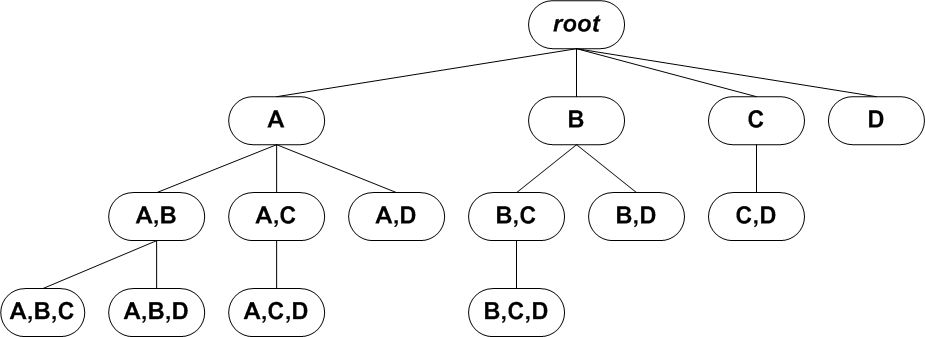
\includegraphics[width = 0.85\columnwidth]{figures/PTS_tree.png}
			\vspace{-0.2cm}
	\caption{PTS search space for $\left\vert T \right\vert = 4$}
	\label{fig:PTS_tree}
			\vspace{-0.2cm}
\end{figure}

We model the entire solution space as a tree (\cref{fig:PTS_tree}) and use a depth-first approach to search the solution space. By \cref{prop:size} we know that we only have to extend the tree up to depth $w.max$ levels for worker $w$. Each node of the tree corresponds to a subset of \emph{T}. Therefore, for any node \emph{n} of the tree, if the corresponding subset of \emph{n} is not in \emph{w.PTS}, according to \cref{prop:subset}, then we can prune the entire sub-tree rooted at \emph{n}.

\begin{algorithm}[h]
\caption{FindPTSs($T, W$)}
\label{algo:FindPTS}
\begin{algorithmic}[1]
\REQUIRE \emph{T} is the set of all tasks and \emph{W} is the set of all workers
\ENSURE \emph{PTSs[]} is the list containing all potential task subsets for different workers.
\FOR{$w$ in $W$}
	\STATE $PTSs[w] = $ SearchBranch($\emptyset, T, w$)
\ENDFOR
\RETURN $PTSs$
\end{algorithmic}
\end{algorithm}

\begin{algorithm}[t]
\caption{SearchBranch($pts, T, w$)}
\label{algo:SearchBranch}
\begin{algorithmic}[1]
\REQUIRE \emph{pts} is the current subset, \emph{T} is the list of remaining tasks and \emph{w} is the worker
\ENSURE \emph{PTSs} is the set of all potential task subsets for \emph{w}
\STATE $PTSs = \emptyset$
\STATE $T_{copy} = T$
\FOR{$t$ in $T$}
	\STATE $T_{copy} = T_{copy} \setminus t$
	\IF{$t$ doesn't temporally overlap with $w$}
		\STATE continue
	\ENDIF
	\STATE $s = pts \cup t$
	\IF{IsPotentialSubset($s, w$)}
		\STATE $PTSs = PTSs \cup s$
		\IF{$\left\vert{s}\right\vert < w.max$ and $T_{copy} \neq \emptyset$}
			\STATE $S =$ Search\_Branch($s, T_{copy}, w$)
			\STATE $PTSs = PTSs \cup S$
		\ENDIF
	\ENDIF
\ENDFOR
\RETURN $PTSs$
\end{algorithmic}
\end{algorithm}

\begin{algorithm}[t]
\caption{IsPotentialSubset($s, w$)}
\label{algo:IsPTS}
\begin{algorithmic}[1]
\REQUIRE $s$ is the input set
\ENSURE $true$ if $s$ is a PTS for $w$ and $false$ otherwise
\FOR{$P$ in PermutationsOf($s$)}
	\STATE $possible = true$
	\STATE $loc = w.l$
	\STATE $time = w.s$
	\FOR{$i=1$ to $\left\vert{P}\right\vert$}
		\STATE $nextTime = $max($P[i].r, time +$ dist($w.l, P[i].l$)
		\IF{$nextTime < P[i].d$ and $nextTime < w.e$}
			\STATE $loc = P[i].l$
			\STATE $time = nextTime$
		\ELSE
			\STATE $possible = false$
			\STATE break
		\ENDIF
	\ENDFOR
	\IF{$!possible$}
		\STATE continue
	\ELSE
		\RETURN $true$
	\ENDIF
\ENDFOR
\RETURN $false$
\end{algorithmic}
\end{algorithm}

\cref{algo:SearchBranch} finds all the PTSs under a specific branch of the search space. The current subset ($pts$) is expanded with a new task ($t$) if $w$ temporally overlaps with $t$ (lines 4-8). If the new subset $s$ is a PTS itself we continue the search for more PTSs in the sub-tree rooted at $s$ (lines  9-15). \cref{algo:IsPTS} checks if a subset $s$ can be a PTS for $w$. According to \cref{def:PTS}, the desired path should start from the current location of $w$ and no sooner than the time the worker becomes available (lines  1-2). We consider all permutations of $s$ and check if a permutation satisfies all the temporal constraints of \cref{def:PTS} (lines 5-14). The subset $s$ will be a PTS only if a permutation is found to satisfy all constraints. Finally in \cref{algo:FindPTS} for each worker we search for PTSs starting the search at the root of the tree.
			
\subsection{Finding the Maximal Matching}
\label{subsec:FindMM}
Having found all PTSs for each worker in step 1, the next step of the algorithm focuses on finding the matching with the maximum value. For this purpose, we construct a graph such that each PTS from step 1 is a vertex in the graph. We call this graph the \emph{PTS-Graph}. Then we show that the \emph{maximum weighted clique} in the PTS-Graph corresponds to the matching with the maximum value.

The PTS-Graph is a multi-layered graph such that for each worker we add a layer to the graph. Withing each layer $l$, for each PTS inside $w_l.PTS$ we add a node to layer $l$. The weight of this node is equal to the value of the corresponding PTS. We use an arbitrary ordering to name the nodes within each layer of the PTS-Graph. Assuming layer $l$ contains $m$ nodes, we name them $n_{l1}$ through $n_{lm}$. Also, we define the set of edges of the PTS-Graph as:
\begin{equation}
E = \left\{ \left\langle n_{ai}, n_{bj} \right\rangle \middle | a \neq b \land \left(PTS_{ai} \cap PTS_{bj} = \emptyset \right) \right\}
\end{equation}
where $PTS_lm$ refers to the corresponding PTS of node $n_{lm}$. In other words, there will be an edge between two nodes in different layers if the corresponding PTSs of the two nodes don't contain the same task.

\begin{figure}[t]
	\centering
	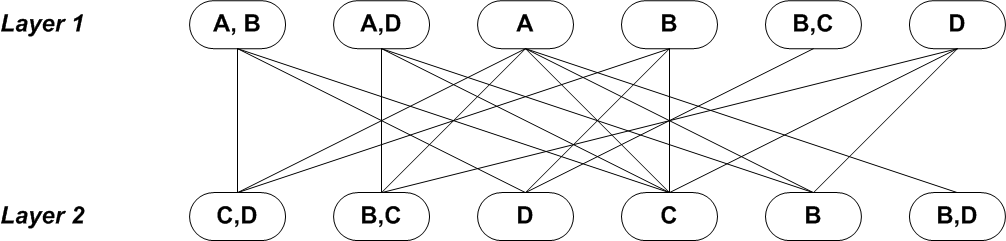
\includegraphics[width = 0.85\columnwidth]{figures/PTS_graph.png}
			\vspace{-0.2cm}
	\caption{A sample two layered PTS-Graph}
	\label{fig:PTS_tree}
			\vspace{-0.2cm}
\end{figure}

Given the PTS-Graph $G(V, E)$, we associate an assignment of tasks to workers with a set of vertices $N \subset V$ as follows: if $n_{lm} \in N$, then every task $t \in PTS_{lm}$ is assigned to $w_l$.

\begin{definition} [Clique]
\label{def:clique}
For undirected graph G=(V,E), a \emph{Clique} in G is a subset $S \subset V$ of vertices, such that $\{x,y\} \in E$ for all distinct $x,y \in S$.
\end{definition}

A clique is said to be \emph{maximal} if its vertices are not a subset of the vertices of a larger clique, and \emph{maximum} if there are no larger cliques in the graph.

\begin{definition} [Maximum Weight Clique]
\label{def:maxClique}
For undirected graph G=(V,E) where each $v \in V$ is assigned a value $w(v)$, the \emph{Maximum Weight Clique} is the clique for which the sum over the weight of all vertices in the clique, is larger than any other clique in the graph.
\end{definition}

It's worth noting that a maximum weight clique is not necessarily a maximum clique but it definitely is a maximal clique.

\begin{theorem}
\label{th:maxClique}
If C* is a maximum weighted clique in the PTS-Graph, then the assignment of tasks to workers corresponding to C*, M*, will be a maximum value matching for the TASC problem.
\end{theorem}

\begin{proof}
Based on the way we generated the PTS graph, no two vertices in C* can contain the same task in their corresponding PTS. Therefore, any task t will be assigned to at most one worker. Next we need to show no other matching M can have a larger value than M*. If such matching M existed, then the clique C corresponding to M, will have a larger weight than C* which conflicts the fact that C* is the maximum weighted clique.
\end{proof}

There exists a vast body of literature on solving the maximum weight clique problem \cite{Kovalyov07}. Here we briefly explain one of these algorithms and refer the interested readers to \cite{Ostergard01}.\\

In \cref{algo:MWC} we start with an arbitrary node ordering. \cite{Ostergard01} suggests a node ordering where $v_1$ is the node with the largest total sum of the weights of its adjacent vertices and so on. \cref{algo:MWC} computes a value $C(k), 1 \leq k \leq n$ which tells the largest weight of a clique, only considering nodes $\left\{v_k, v_{k+1}, ..., v_n\right\}$. If $w(i)$ denotes the weight of $v_i$, then we will have $C(n) = w(i)$ and other values for $C()$ are computed in a backtrack search. For $1 \leq k \leq n-1, C(k) > C(k+1)$ only when a corresponding clique exists and contains $v_k$. If such clique does not exist then $C(k) = C(k+1)$. In order to find such $C(k)$ clique, a branch and bound approach is used to search all possible cliques. Details of the branch and bound algorithm can be found in \cite{Ostergard01}.

\begin{algorithm}
\caption{MaximumWeightClique($V, E$)}
\label{algo:MWC}
\begin{algorithmic}[1]
\REQUIRE $V$ is an ordering of the nodes and $E$ is the set of edges in the graph
\ENSURE $C$ a subset of $V$ as the maximum weighted clique
\STATE $C = \left\{ v_n \right\}$
\STATE $max = w(n)$
\FOR{$k: n-1$ down to $1$}
	\STATE $\left\langle C_k, w \right\rangle =$ FindMaxClique($V, E, v_k$)
	\IF{$w > max$}
		\STATE $C = C_k$
		\STATE $max = w$
	\ENDIF
\ENDFOR
\RETURN $C$
\end{algorithmic}
\end{algorithm}

\subsection{Complexity Analysis}
\label{subsec:exactcomplexity}

Here we analyze the time complexity of our proposed exact algorithm. For simplicity we assume $\left\vert T \right\vert = n$, $\left\vert W \right\vert = m$ and $\left\vert w.max \right\vert = p$. We start with \cref{algo:IsPTS}. The size of set $s$ is at most equal to $p$, hence the number of permutations of $s$ is $O(p^p)$. Also the for loop in line 5 will run at most $p$ times which will make the overall complexity of \cref{algo:IsPTS} $O(p^{p+1})$. For \cref{algo:SearchBranch} we can assume that we are running the IsPotentialPTS() method for each node of the search space tree(\cref{fig:PTS_tree}) once. At level $i$ of the search space tree we will have at most $C(n,i)$. Also for each node in level $i$ the size of the task subsets will be $i$. Hence, the IsPotentialSubset() method will run in $O(i^{i+1})$. Therefore the amortized time complexity of \cref{algo:SearchBranch} will be:

\begin{equation*}
\mathlarger{\mathlarger{\sum}}_{i = 1}^{p} \dbinom{n}{i} O(i^{i+1}) = O(n^{n-p}p^{p+1})
\end{equation*}

Since we run the SearchBranch method for each worker once in, we can conclude the the time complexity of \ref{algo:FindPTS} is $O(mn^{n-p}p^{p+1})$.\\

In \cref{algo:MWC} we implement the FindMaxClique() method, we use a branch and bound algorithm described in \cite{Ostergard01}. The time complexity of this algorithm will be $O(n^n)$ for a graph of size $n$. Therefore, for a graph of size $n$, the overall time complexity of \cref{algo:MWC} will be $O(n^{n+1})$.\\

We end the section with a discussion on how generalizing the spatial crowdsourcing framework can affect the algorithm introduced in this section. In \cite{Kazemi13} it's assumed that each task requires a certain level of \emph{confidence} and only workers with a \emph{trust} level higher than than will be able to perform the task. It's also seen that in some spatial crowdsouring frameworks, workers define a spatial range and only perform task within this range. Constraints like this will only remove a subset of tasks from the list of tasks a certain worker is able to execute. As a result, the search space of \cref{algo:FindPTS} will get reduced and we end up with few number of PTSs per worker. This in turn will reduce the size of the PTS-Graph in \cref{subsec:FindMM}.

\section{Approximate Clairvoyant Algorithms}
\label{sec:approxalgo}

The algorithm presented in \cref{sec:exactalgo} is computationally expensive to run. In this section we present a greedy algorithm for solving the TASC problem. We use two rather simple heuristics; (1) We give priority to tasks with higher values and (2) among different workers that can execute task $t$, we select the worker which is closest to $t$. The logic behind heuristic (1) is to assign tasks with larger benefit gains first in order to maximize the overall benefit. We can see similar heuristics in many job scheduling problems \cite{Kolen07}. As for the second heuristic, we try to assign tasks to nearby workers so the amount of time spent to execute a specific task is minimized. This is turn will leave the worker with more time to execute other tasks.

\begin{algorithm}[h]
\caption{MostValuableFirst($W, T$)}
\label{algo:MVF}
\begin{algorithmic}[1]
\REQUIRE $W$ is the set of workers and $T$ is the set of tasks
\ENSURE $M$ is a set of assignments between tasks and workers
\STATE $M = \emptyset$
\STATE $T_{sorted} = $ Sort $T$ based on $t.v$
\WHILE{$T_{sorted} \neq \emptyset$}
	\STATE $W_t = W$
	\WHILE{$W_t \neq \emptyset$}
		\STATE $w = w \in W_t$ with minimum distance to $t$
		\IF{IsPotentialSubset($w.T \cup t, w$)}
			\STATE assign $t$ to $w$.
			\STATE $M = M \cup \left\langle w, t \right\rangle$
			\IF{$\left\vert w.T \right\vert = w.max$}
				\STATE $W = W \setminus w$
			\ENDIF
		\ELSE
			\STATE $W_t = W_t \setminus w$
		\ENDIF
	\ENDWHILE
\ENDWHILE
\RETURN $M$
\end{algorithmic}
\end{algorithm}

\cref{algo:MVF} outlines the implementation of these heuristics. In line 2, we sort the tasks based on their values in accordance with heuristic (1). For the sort method, we break ties by giving a higher priority to tasks with smaller distance to their nearest worker. This means that if two task have equal values, the one with smaller distance to its nearest worker will have a higher priority. In this way, the MostValuableFirst() method will work perfectly fine in the case all tasks have similar value and the goal is to only maximize the number of assigned tasks.\\

In line 7 of \cref{algo:MVF} we use the IsPotentialSubset() method described in \cref{algo:IsPTS}. In \cref{subsec:exactcomplexity} we showed that the complexity of \cref{algo:IsPTS} is $O(p^{p+1})$. This can make \cref{algo:MVF} computationally expensive to run which contradicts the goal of implementing a fast heuristic algorithm. In the case of larger values of $p$, instead of the exact solution proposed in \cref{algo:IsPTS}, we can use several approximate algorithms that have been proposed for vehicle routing problems. Depending on the desired accuracy we seek to achieve, these algorithm can run as fast as $O(p)$ \cite{Laporte00}.


\section{Spatial Distribution}

Spatial Distribution

\section{Experiments}
\label{sec:experiments}
Unlike regular crowdsourcing, there is no publicly available platform for running real-world spatial crowdsourcing campaigns. With platforms such as Amazon Mechanical Turk, workers do not perform spatial crowdsourcing tasks. For this reason, we simulated various spatial crowdsourcing campaigns on an Inter(R) Core(TM)2 Duo 3.16GHz PC with 4GB memory running Microsoft Windows 7.

\subsection{Dataset}
\label{subsec:dataset}
Due to its commercial value, real-life SC systems such as Uber and TaskRabbit do not make their datasets available to public. However, we were able to use a large collection of geo-tagged images from Flickr \cite{Thomee15} as an input to Auction-SC. The dataset consists of \textasciitilde 15 million images with attributes such as location, time taken, time uploaded, the user who took the picture, etc.

We correspond each image with a spatial task considering that the task was to take a photo at a specific location. We set the deadline of the task to the time the image was taken and the duration of the task to the interval between the time the image was taken and the time it was uploaded. Each user in the dataset corresponds to a worker. The original location of the worker is randomly selected. The worker is available during the interval between the first time he took a photo and the last time he uploaded one. We ran 5 separate instances, each of which with images in a different metropolitan area. \cref{tab:flickr_stats} shows the total number of tasks (and workers) for each city.

\begin{table}[h]
\begin{center}
\begin{tabular}{| l || c | c |} \hline
			&	\# of Tasks	&	\# of Workers	\\ \hline
Los Angeles	&	219,332		&		19,081		\\ \hline
New York	&	390,229		&		17,603		\\ \hline
London		& 	366,034		&		18,480		\\ \hline
Paris		&	237,344		&		14,275		\\ \hline
Beijing		&	23,335		&		1,598		\\ \hline
\end{tabular}
\vspace{-0.1in}
\caption{\small{Number of tasks/worker for each city in Flickr dataset}}
\label{tab:flickr_stats}
\end{center}
\end{table}

We also generated a synthetic dataset with realistic streaming workload based on the methodology proposed in \cite{Tang07}. To generate a workload suitable for SC systems we modeled three different sets of parameters:

\noindent \textbf{Temporal Parameters:} In \cite{Basu15}, it is shown that with crowdsourcing environments, workers and tasks arrive following Poisson processes \cite{Stoyan87}.The default Poisson arrival rates for tasks and workers are $\mu_t = 20/min$ and $\mu_w = 3/min$, respectively. Subsequently, the duration of the tasks and workers were randomly sampled from closed range of $\left[1,4 \right]$ hours and $\left[1,8 \right]$ hours, respectively.

\noindent \textbf{Spatial Parameters:} \cref{fig:la_flickr} shows the spatial distribution of tasks from our real-world dataset in Los Angeles. As depicted, the tasks are not uniformly distributed in space. The spatial distribution is rather skewed, meaning that the density of the tasks at certain areas is higher. To model the same behavior with our synthetic workloads, we created 6 two dimensional Gaussian clusters with randomly selected means and standard deviations. Eighty percent of the tasks are sampled within the clusters and the rest are uniformly distributed.

\noindent \textbf{Static Parameters:} In addition to the spatiotemporal parameters, we consider two other parameters. The default \emph{workload size} of each experiment is 10K tasks. The task arrival rate and the number of tasks determine the duration of the simulation. Based on the duration of the simulation and the worker arrival rate, the total number of workers may vary.\\
The maximum number of tasks a worker can perform, i.e., $w_{max}$, is a uniformly random number from the closed interval $\left[8,12 \right]$.

\begin{figure}[h]
	\centering
	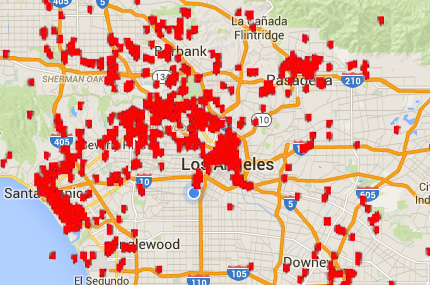
\includegraphics[scale=0.35]{figures/la_flickr.jpg}
	\caption{Spatial Distribution of Tasks in Flickr}\label{fig:la_flickr}
\end{figure}

%\subsection{Online vs. Offline}
%As the first set of experiments, we compare how the results of the real-time algorithms compare with the optimal solution computed using the offline clairvoyant algorithm explained in \cref{sec:exactalgo}. Because of the high complexity of the offline algorithm, we are not able to run tests with large workloads and thus we use workloads with 100 tasks. The experimental results of \cref{fig:off_vs_on} show that the best real-time algorithms perform close to \textasciitilde 60\% of the optimal solution. Our results are consistent with studies that compute a \emph{competitive ratio} \cite{Sleator85} of $1 - e^{-1}$ for the online matching problem with random inputs \cite{Goel08}.

%\begin{figure}[h]
%	\centering
%	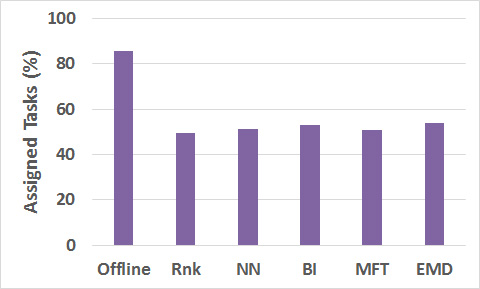
\includegraphics[width = 0.6\columnwidth]{figures/off_vs_on.jpg}
%	\caption{Comparison of Offline and Real-time approaches}\label{fig:off_vs_on}
%\end{figure}

\subsection{Assignment Quality}
In this section we evaluate the quality of the assignments using different real-time non-clairvoyant algorithms. First, we compare them using the Flickr and the synthetic datasets. Subsequently, using the synthetic datasets, we show how the spatial and temporal settings of the problem can affect the performance of the real-time assignment quality.

\begin{figure}[h]
    \centering
    \subfigure[Flickr]{
        \label{fig:quality_real}
        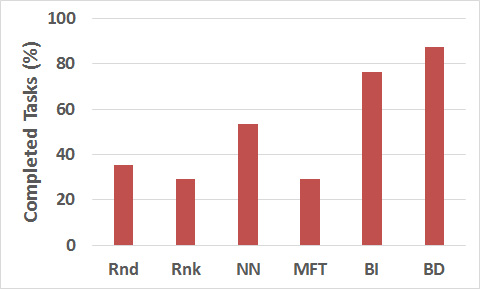
\includegraphics[width = 0.45\columnwidth]{figures/quality_real.jpg}
    }
    \subfigure[Synthetic]{
        \label{fig:quality_syn}
        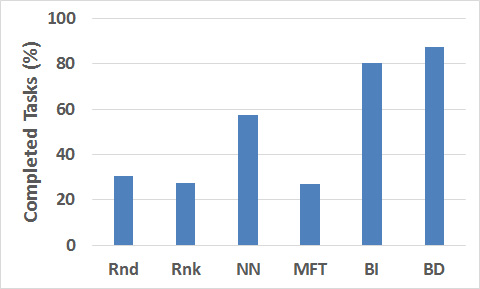
\includegraphics[width = 0.45\columnwidth]{figures/quality_syn.jpg}
    }
    \vspace{-0.15in}
    \caption{Assignment Quality of Real-Time Approaches}
    \label{fig:quality}
\end{figure}

\cref{fig:quality} compares the assignment quality of different real-time algorithms. As we can see, both SC approaches outperforms the best non-SC algorithm by almost 25\%. The main reason as explained in \cref{sec:onlinealgo} is that, the SC rules perform scheduling when matching tasks with workers. Furthermore, the BD approach outperforms BI by at most 10\%. This is not surprising as BD tends to ``move" workers to areas where future tasks are more likely to appear, thus achieving higher assignment in long term. Among the non-SC approaches NN outperforms other rules by almost 2 times more completed tasks. The reason MFT does not outperform baseline approaches (Rnd and Rnk) can be explained by what we call a \emph{radical move}. A \emph{radical move} is when the SC-Server assigns a task to a worker which requires it to move a relatively long distance to reach the location of that task. Since we do not consider any spatial proximity to the task with MFT, there is a high chance to end up with assignments resulting in radical moves. With NN and BI the general idea is to prevent radical moves as much as possible. With BD, although radical moves occur, but only if the worker moves to areas where there will be more tasks to complete. 

\begin{figure}[h]
    \centering
    \subfigure[Rnd]{
        \label{fig:rnd_comp}
        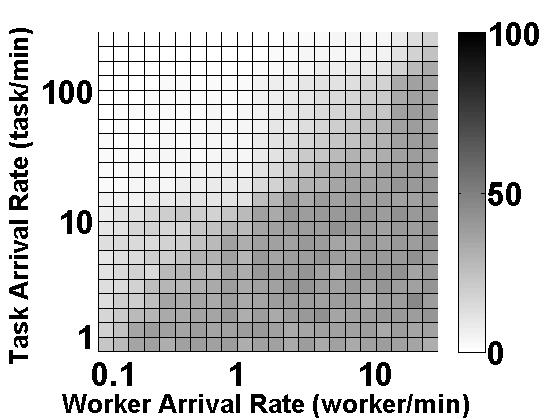
\includegraphics[width = 0.45\columnwidth]{figures/rnd.jpg}
    }
    \subfigure[Rnk]{
        \label{fig:rnk_comp}
        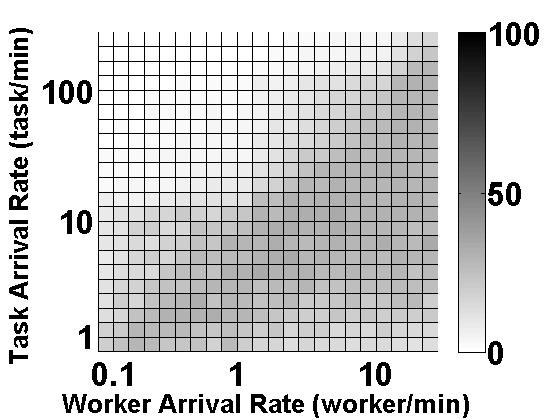
\includegraphics[width = 0.45\columnwidth]{figures/rnk.jpg}
    }
    \subfigure[MFT]{
        \label{fig:mft_comp}
        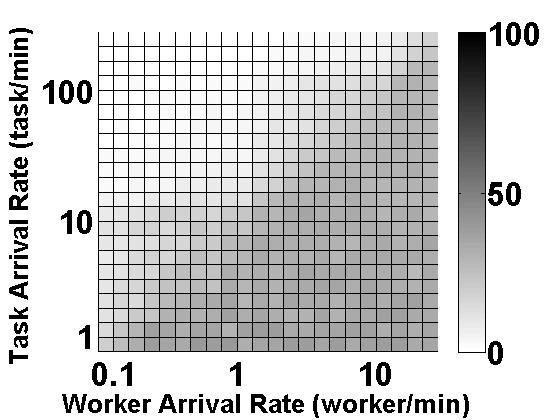
\includegraphics[width = 0.45\columnwidth]{figures/mft.jpg}
    }
    \subfigure[NN]{
        \label{fig:nn_comp}
        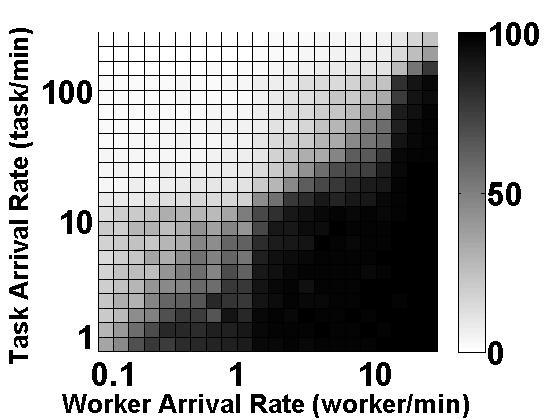
\includegraphics[width = 0.45\columnwidth]{figures/nn.jpg}
    }
    \subfigure[BI]{
        \label{fig:bi_comp}
        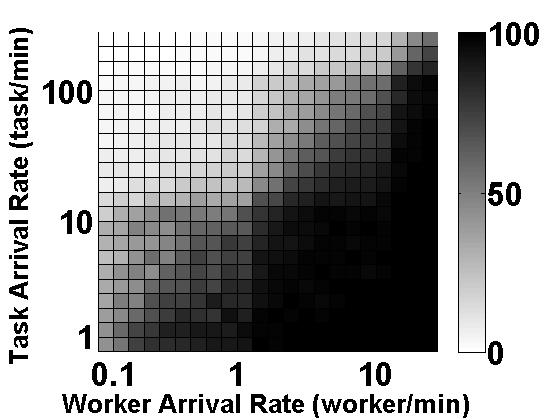
\includegraphics[width = 0.45\columnwidth]{figures/bi.jpg}
    }
    \subfigure[BD]{
        \label{fig:emd_comp}
        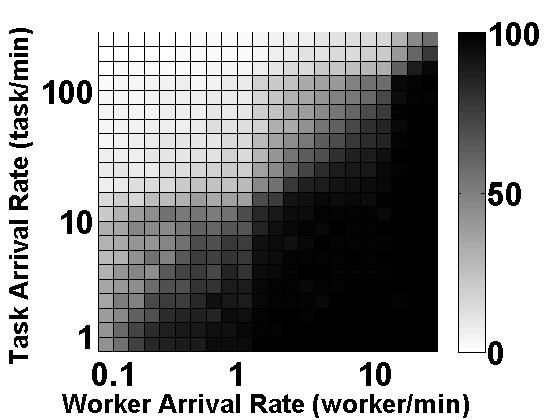
\includegraphics[width = 0.45\columnwidth]{figures/emd.jpg}
    }
    \vspace{-0.15in}
    \caption{\small{Assignment Profile-Varying Worker/Task Arrival Rates}}
    \label{fig:tw_rate}
\end{figure}

In order to study the effect of temporal parameters of SC, we ran several experiments using different pairs of task arrival rates ($t_{rate}$) and worker arrival rates ($w_{rate}$). In \cref{fig:tw_rate} we show the effect of increasing $t_{rate}$ and $w_{rate}$ on the quality of the assignment. The level of grayness corresponds to the percentage of completed tasks with black and white representing 100\% and 0\%, respectively. As we can see with small number of workers, as we increase the task arrival rate, the percentage of completed tasks decreases where at the top left corner of each plot we get close to 0\%. On the other hand in \cref{fig:nn_comp,fig:bi_comp,fig:emd_comp} for NN, BI and BD, with small number of incoming tasks, as we increase $w_{rate}$, eventually all tasks will be completed. \cref{fig:tw_rate} clearly shows that NN, BI and BD outperform Rnd, Rnk and MFT independent of the $t_{rate}$ and $w_{rate}$.

\begin{figure}[h]
	\centering
	\subfigure[BI Vs. NN]{
        \label{fig:bi_nn}
        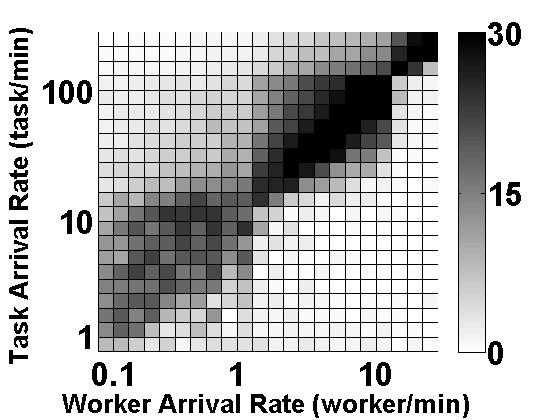
\includegraphics[width = 0.45\columnwidth]{figures/bi_nn.jpg}
    }
    \subfigure[BD Vs. NN]{
        \label{fig:emd_nn}
        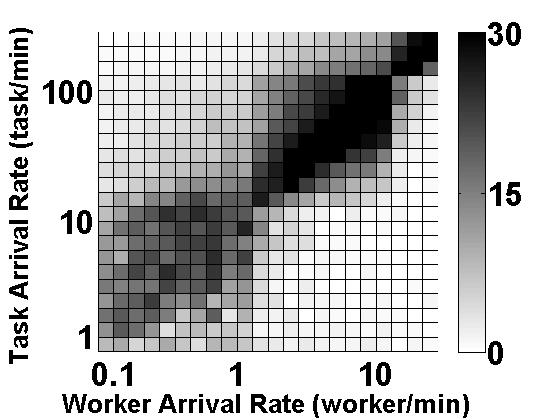
\includegraphics[width = 0.45\columnwidth]{figures/emd_nn.jpg}
    }
    \subfigure[BD Vs. BI]{
        \label{fig:emd_bi}
        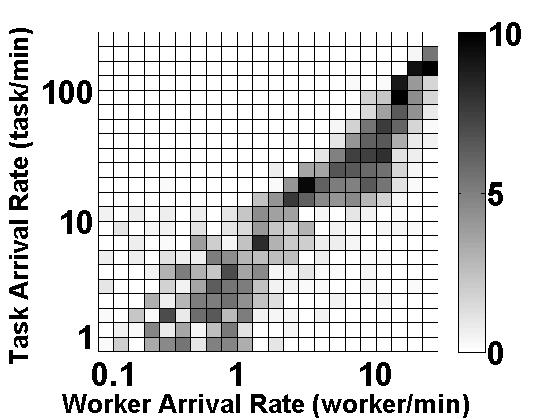
\includegraphics[width = 0.45\columnwidth]{figures/emd_bi.jpg}
    }
    \vspace{-0.15in}
	\caption{\small{Assignment Difference-Varying Worker/Task Arrival Rates}}\label{fig:rate_comp}
\end{figure}

To better evaluate the leading real-time approaches, NN, BI and BD, in \cref{fig:rate_comp} we performed a pair-wise comparison by taking their task completion rates. For example, \cref{fig:bi_nn} shows the difference between BI and NN. We observe that these three approaches perform similarly at the two extreme cases discussed in \cref{fig:tw_rate}, i.e., high task-low worker and low task-high worker. BI and BD outperform NN up to 30\% when the problem is more complex, i.e., outside the extreme cases. An interesting observation in \cref{fig:bi_nn,fig:emd_nn} is that BI and BD outperform NN by a much larger margin at scale (higher $t_{rate}$ and $w_{rate}$). The reason is that with higher higher $t_{rate}$ and $w_{rate}$ more workers are moving around and more tasks come and leave so in general the spatiotemporal dynamism of the system increases. BI and BD cope with the dynamism by guaranteeing a task gets assigned to worker that can complete it. On the contrary, NN ignores the schedule of a worker during matching and this becomes more important as there is more dynamism in the system.

\begin{figure}[h]
	\centering
	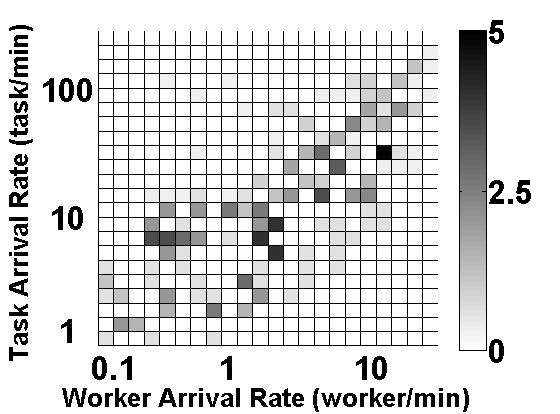
\includegraphics[scale=0.25]{figures/bi_abi.jpg}
	\vspace{-0.1in}
	\caption{Assignment Difference of BI Vs. ApproxBI}\label{fig:bi_abi}
\end{figure}

We mentioned earlier that with the SC-rules, the workers perform an exhaustive search to find out if they can fit a new task into their schedule. As workers accept new tasks, they also complete some other tasks so as we observed in our experiments, performing an exhaustive search did not cause any scalability issues. Nevertheless, one might want to replace the exhaustive search with a polynomial time approximate algorithm. With ApproxBI, we use the insertion algorithm from \cite{Rosenkrantz74} that runs in $O(n^2)$. \cref{fig:bi_abi} shows the change affects the quality of the assignment by less than 5\%. The difference caused by ApproxBI is that the workers that are eligible for a task using BI, may not be able to fit the task in their schedules using ApproxBI due to the approximation. As a result, using ApproxBI the server may not be able to assign some tasks even if they can be completed using BI. Fortunately, as shown in \cref{fig:bi_abi}, that does not happen very often regardless of $t_{rate}$ and $w_{rate}$.

The next set of experiments compare the effect of the spatial distribution of tasks. We compared the quality of the final assignment for three different distribution. Even though real-world data usually follow a skewed spatial distribution (\cref{subsec:dataset}), the results of these experiments show that regardless of the distribution, SC rules outperform non-SC rules. With the first distribution, the location of the tasks follow a spatial Poisson process \cite{Baddeley07}. The other two distributions are a Uniform 2D distribution and a Skewed distribution. The results in \cref{fig:dists} show that SC rules generate assignments at least 20\% better than non-SC rules. Also, we can see with Poisson and Uniform distributions, there is not much difference between BI and EMD. The reason is that both distributions generate tasks at completely random locations. Consequently, tasks are released at every area with the same probability and hence EMD and BI become similar.

\begin{figure}[h]
	\centering
	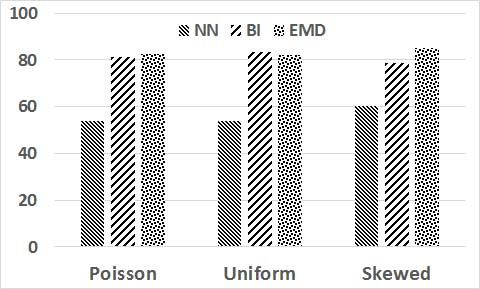
\includegraphics[scale=0.25]{figures/dists.jpg}
	\vspace{-0.1in}
	\caption{Assignment Difference-Varying Distribution}\label{fig:dists}
\end{figure}

The final set of experiments regarding assignment quality, compare bathed assignment with online assignment results. For batched assignment we used the LALS algorithm from \cite{Deng15} \footnote{The reported runtimes in \cite{Deng15} outperform those of \cite{Chen15}}.

\begin{figure}[h]
	\centering
	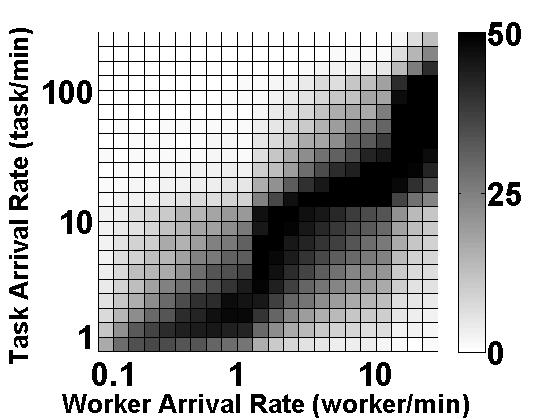
\includegraphics[scale=0.25]{figures/bi_lals.jpg}
	\vspace{-0.1in}
	\caption{Assignment Difference of BI Vs. LALS}\label{fig:bi_lals}
\end{figure}

Earlier we explained for some use cases (e.g., Uber), batched assignment does not even satisfy application requirements. Nevertheless, the results in \cref{fig:bi_lals} show even if non real-time assignments are tolerable, the quality of batched assignment is not as good as the online assignment. One reason is that the LALS algorithm performs the matching phase and then attempts to schedule tasks for their matched workers. All tasks that could not be scheduled for their matched workers, will go back to the matching phase and the process continues until all tasks are scheduled or there is no more worker to match with a task. When performing the matching, the schedule of the worker is not considered and hence a task might end up getting matched to and scheduled for a worker that was not the best worker. This in turn, can lower the chances of that worker to get assigned to a new task in the future. The second reason is that while a task is waiting at the server to get processed with the next batch, depending on the length of the batching time interval, it will lose some portion of its availability time which in turn, can lower the chances of the task fitting a worker's schedule.

\subsection{Scalability}
The last set of experiments focus on measuring the scalability of two system architectures, i.e., centralized and Auction-SC (decentralized). We compare the scalability of the real-time Auction-SC algorithms with the equivalent implementation of the same algorithms on a single centralized SC-Server. 

We can measure the scalability of SC systems by their throughput: the number of tasks processed per second , or equivalently, the processing time per task, shown in \cref{fig:runtime}. Because of the decentralized architecture of Auction-SC, in \cref{fig:runtime} we see that the average processing time of a single task does not change as the arrival rate of workers increases. On the contrary, with the centralized architecture, the average processing time of a single task increases linearly as we increase the number of workers and is several orders of magnitude higher than Auction-SC approaches. Although BD consumes more time than other real-time algorithms, but only takes up to 3 milliseconds.

\begin{figure}[h]
    \centering
    \subfigure[\emph{\small{wRate = 1 worker/min}}]{
        \label{fig:runtime_50}
        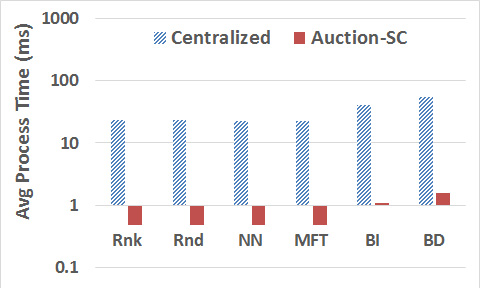
\includegraphics[width = 0.45\columnwidth]{figures/run_time_50.jpg}
    }
    \subfigure[\emph{\small{wRate = 2 worker/min}}]{
        \label{fig:runtime_100}
        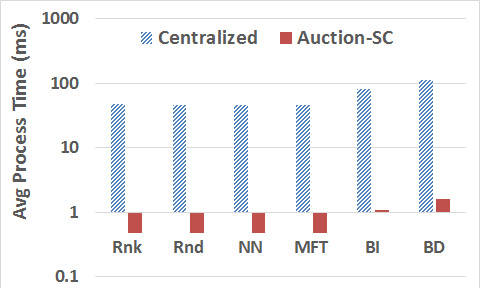
\includegraphics[width = 0.45\columnwidth]{figures/run_time_100.jpg}
    }
    \subfigure[\emph{\small{wRate = 4 worker/min}}]{
        \label{fig:runtime_200}
        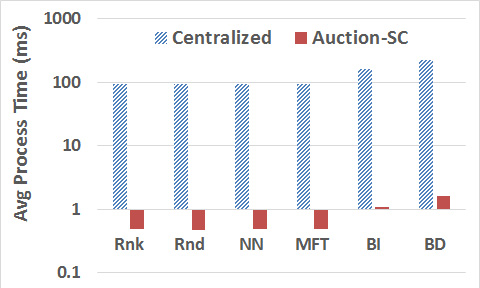
\includegraphics[width = 0.45\columnwidth]{figures/run_time_200.jpg}
    }
    \subfigure[\emph{\small{wRate = 8 worker/min}}]{
        \label{fig:runtime_400}
        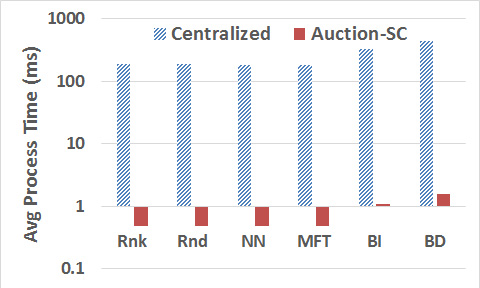
\includegraphics[width = 0.45\columnwidth]{figures/run_time_400.jpg}
    }
       \vspace{-0.15in}
    \caption{Average processing time for a single task}
    \label{fig:runtime}
\end{figure}

For a \emph{CEP} engine, it is also common to measure the queuing delay of events \cite{Wu06} once they arrive at the system as a metric for the scalablility of the systems. In \cref{fig:queue} we compare the average queuing delay of tasks in the two architectures after running them for 1 hour. We can see that the centralized system suffers from queuing delays with less than 10 tasks/second. On the other hand, with Auction-SC, even for BD, we do not observe queuing delays for up to 500 tasks/second. \textcolor{red}{To give a better perspective, in \cref{fig:req} we compare the scalability of the centralized and Auction-SC approaches with the current requirements of a ride sharing application in New York City \cite{NYCTaxi} for BI and BD bidding rules. As shown, while a centralized server is not able to satisfy the current requirements, Auction-SC can scale orders of magnitudes higher than what currently is needed.} \cref{fig:queue_auc} also shows that BD incurs higher delay than BI but results in higher completion rates (\cref{fig:quality,fig:rate_comp}). Users of Auction-SC can choose between BD and BI to balance their needs for assignment quality and efficiency.

\begin{figure}[h]
    \centering
    \subfigure[\emph{\small{Centralized}}]{
        \label{fig:queue_cent}
        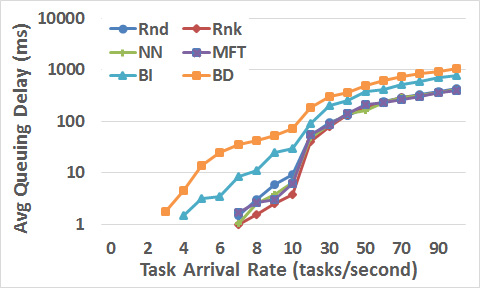
\includegraphics[width = 0.65\columnwidth]{figures/queue_cent.jpg}
    }
    \subfigure[\emph{\small{Auction-SC}}]{
        \label{fig:queue_auc}
        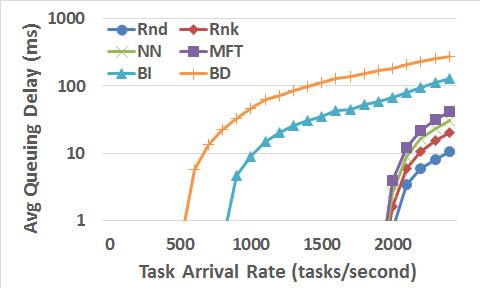
\includegraphics[width = 0.65\columnwidth]{figures/queue_auc.jpg}
    }
    \vspace{-0.15in}
    \caption{Average queuing delay}
    \label{fig:queue}
\end{figure}

\begin{figure}[h]
	\centering
	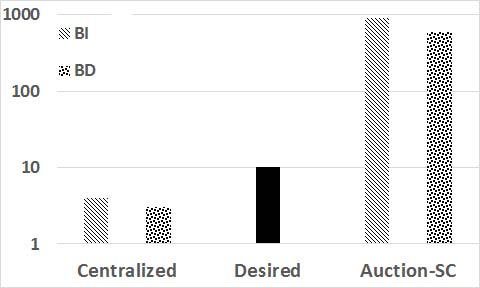
\includegraphics[scale=0.25]{figures/scale_req.jpg}
	\vspace{-0.1in}
	\caption{Centralized and Auction-SC Vs. Desired Scalability}\label{fig:req}
\end{figure}

To summarize the results of our experiments, we showed that when SC bidding rules are used, the quality of the assignment is much higher as compared to when a non-SC rule is used. The consideration of scheduling at the time a task is being matched is the main reason for the better overall assignments. When running on a single centralized SC-Server, neither one of bidding rules can scale. Furthermore, the time required to process a single task increases linearly as more workers are added to the system in a centralized architecture. Scalability of a single centralized server suffers more when SC bidding rules are used due to their higher computation complexity. However, with Auction-SC we solve the scalability problem by splitting the scheduling and matching responsibilities between workers and the SC-Server. Consequently, Auction-AC can afford to execute complex SC bidding rules, resulting in a very high quality assignment. %\cref{tab:summary} shows the summary of our experimental results.

%\begin{table*}
%  \centering
%  \begin{tabular}{|c|c|c|c|c|c|c|c|c|}
%    \hline
%    \multicolumn{2}{|>{\columncolor{kugray5}}c|}{}&\multicolumn{4}{c|}{non-SC bidding rules}&\multicolumn{2}{c|}{SC bidding rules}\\
%    \arrayrulecolor{kugray5}
%    \arrayrulecolor{black}
%    \cline{3-8}
%    \multicolumn{2}{|>{\columncolor{kugray5}}c|}{}&Rnd&Rnk&NN&MFT&BI&BD\\
%    \hline
%    \multirow{2}{*}{Centralized}&Scalability&Bad&Bad&Bad&Bad&Very Bad&Very Bad\\
%    \cline{2-8}
%                         		&Assignment Quality&Very Bad&Very Bad&Bad&Very Bad&Very Good&Very Good\\
%    \hline
%    \multirow{2}{*}{Auction-SC}&Scalability&Very Good&Very Good&Very Good&Very Good&Good&Good\\
%    \cline{2-8}
%                         		&Assignment Quality&Very Bad&Very Bad&Bad&Very Bad&Very Good&Very Good\\
%    \hline
%  \end{tabular}
%  \vspace{-0.1in}
%  \caption{Summary of Experimental Results}
%  \label{tab:summary}
%\end{table*}

\section{Conclusion and Future Work}
\label{sec:future}

In this paper, we studied the problem of real-time task assignment and scheduling in spatial crowdsourcing. We showed that neither of the two current approaches for task assignment in spatial crowdsourcing, batched assignment and centralized online assignment, can scale as either task matching or task scheduling will become the bottleneck. Therefore, we introduced an auction-based framework in which we split the matching and scheduling responsibilities between SC-Server and workers, respectively. We showed that by exploiting the spatiotemporal aspects of SC, with our proposed algorithms, the workers will be able to complete up to 30\% more tasks as compared to non-SC approaches. The decentralized architecture of our framework allows for performing such high quality assignments at scale.

In this paper, we assumed each task can be performed instantaneously, e.g., taking a picture. Once that assumption is relaxed, we will face new challenges with scheduling the tasks. We also assumed each task requires the worker to travel to a single location. However, in other applications the worker may need to visit multiple locations for a single task, e.g., in the Uber application the worker has to pick up a passenger at one location and drop him off at a second location. We plan to extend our Auction-SC framework to incorporate these two features.

\begin{scriptsize}
\bibliographystyle{IEEEtran}
\bibliography{spatialcrowdsourcing}
\end{scriptsize}

\end{document}